\documentclass[10pt]{exam}

\usepackage{amssymb, amsmath, amsthm, mathrsfs, multicol, graphicx}
\usepackage{tikz}

 \def\d{\displaystyle}
\def\?{\reflectbox{?}}
\def\b#1{\mathbf{#1}}
\def\f#1{\mathfrak #1}
\def\c#1{\mathcal #1}
\def\s#1{\mathscr #1}
\def\r#1{\mathrm{#1}}
\def\N{\mathbb N}
\def\Z{\mathbb Z}
\def\Q{\mathbb Q}
\def\R{\mathbb R}
\def\C{\mathbb C}
\def\F{\mathbb F}
\def\A{\mathbb A}
\def\X{\mathbb X}
\def\E{\mathbb E}
\def\O{\mathbb O}
\def\U{\mathcal U}
\def\pow{\mathcal P}
\def\inv{^{-1}}
\def\nrml{\triangleleft}
\def\st{:}
\def\~{\widetilde}
\def\rem{\mathcal R}
\def\sigalg{$\sigma$-algebra }
\def\Gal{\mbox{Gal}}
\def\iff{\leftrightarrow}
\def\Iff{\Leftrightarrow}
\def\land{\wedge}
\def\And{\bigwedge}
\def\AAnd{\d\bigwedge\mkern-18mu\bigwedge}
\def\Vee{\bigvee}
\def\VVee{\d\Vee\mkern-18mu\Vee}
\def\imp{\rightarrow}
\def\Imp{\Rightarrow}
\def\Fi{\Leftarrow}

%\def\={\equiv}
\def\var{\mbox{var}}
\def\mod{\mbox{Mod}}
\def\Th{\mbox{Th}}
\def\sat{\mbox{Sat}}
\def\con{\mbox{Con}}
\def\bmodels{=\joinrel\mathrel|}
\def\iffmodels{\bmodels\models}
\def\dbland{\bigwedge \!\!\bigwedge}
\def\dom{\mbox{dom}}
\def\rng{\mbox{range}}
\DeclareMathOperator{\wgt}{wgt}


\def\bar{\overline}


\newcommand{\vtx}[2]{node[fill,circle,inner sep=0pt, minimum size=4pt,label=#1:#2]{}}
\newcommand{\va}[1]{\vtx{above}{#1}}
\newcommand{\vb}[1]{\vtx{below}{#1}}
\newcommand{\vr}[1]{\vtx{right}{#1}}
\newcommand{\vl}[1]{\vtx{left}{#1}}
\renewcommand{\v}{\vtx{above}{}}

\def\circleA{(-.5,0) circle (1)}
\def\circleAlabel{(-1.5,.6) node[above]{$A$}}
\def\circleB{(.5,0) circle (1)}
\def\circleBlabel{(1.5,.6) node[above]{$B$}}
\def\circleC{(0,-1) circle (1)}
\def\circleClabel{(.5,-2) node[right]{$C$}}
\def\twosetbox{(-2,-1.4) rectangle (2,1.4)}
\def\threesetbox{(-2.5,-2.4) rectangle (2.5,1.4)}
\newcommand{\twoline}[2]{\begin{pmatrix}#1 \\ #2 \end{pmatrix}}


\def\circleA{(-.5,0) circle (1)}
\def\circleAlabel{(-1.5,.6) node[above]{$A$}}
\def\circleB{(.5,0) circle (1)}
\def\circleBlabel{(1.5,.6) node[above]{$B$}}
\def\circleC{(0,-1) circle (1)}
\def\circleClabel{(.5,-2) node[right]{$C$}}
\def\twosetbox{(-2,-1.5) rectangle (2,1.5)}
\def\threesetbox{(-2,-2.5) rectangle (2,1.5)}

%\pointname{pts}
\pointsinmargin
\marginpointname{pts}
\addpoints
\pagestyle{head}
\printanswers

\firstpageheader{Math 228}{\bf Homework 7 Solutions}{Due: Wednesday, October 17}


\begin{document}
% \noindent \textbf{Instructions}: Same rules as usual.  Turn in solutions on separate pages, and do not consult the internet.

\begin{questions}

\question[9] How many triangles can you draw using the dots below as vertices?

\begin{center}
	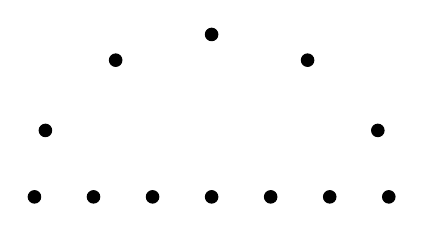
\begin{tikzpicture}[scale=.75]
		\foreach \x in {-3,...,3}{
		\draw[fill] (\x,.5) circle (3pt);
		}
		\foreach \x in {-2,...,2}{
		\draw[fill] (90+\x*30:3.25) circle (3pt);
		}
	\end{tikzpicture}
	\begin{parts}
		\part Find an expression for the answer which is the sum of three terms involving binomial coefficients.  Hint: how many vertices can be on the horizontal axis?
		\begin{solution}
			Any triangle will have 2, 1 or 0 vertices on the bottom row of vertices.  If there are 2 vertices on the bottom row, there are $\binom{7}{2}$ ways to choose these, and for each, there are $5 = \binom{5}{1}$ choices for the third vertex.  So there are $\binom{7}{2}\binom{5}{1}$ such triangles.

			There are $\binom{7}{1}\binom{5}{2}$ triangles with 1 vertex among the 7 on the bottom row (and 2 among the 5 in the semi-circle).  There are $\binom{7}{0}\binom{5}{3}$ that have all three vertices in the semi-circle (and 0 among the 7 on the bottom row).

			Thus the number of triangles is
			\[\binom{7}{0}\binom{5}{3}+\binom{7}{1}\binom{5}{2} + \binom{7}{2}\binom{5}{1}.\]
		\end{solution}
		\part Find an expression for the answer which is the difference of two  binomial coefficients.  Hint: will \emph{any} three dots work as the vertices?
		\begin{solution}
			What if we pick three of the seven vertices?  Most of these choices will determine a unique triangle (and every triangle will correspond to a choice of three vertices).  This can be done in $\binom{12}{3}$ ways.  However, if we picked all three from the bottom row, then we would not get a triangle, so we need to subtract all these $\binom{7}{3}$ ways.  Thus the number of triangles is
			\[\binom{12}{3} - \binom{7}{3}\]
		\end{solution}
		\part Generalize the above to state and prove a binomial identity using a combinatorial proof.  Say you have $x$ points on the horizontal axis and $y$ points in the semi-circle.
		\begin{solution}
			We will prove the binomial identity:
			\[\binom{x}{0}\binom{y}{3} + \binom{x}{1}\binom{y}{2} + \binom{x}{2}\binom{y}{1} = \binom{x+y}{3} - \binom{x}{3}.\]
			A combinatorial proof consists of a question which can be answered as the left hand side and also as the right hand side.

			\begin{proof}
				Consider the counting question, ``How many triangles can you form using a horizontal row of $x$ points sitting below a semi-circle of $y$ points?''

				One way to answer this question is to divide the triangles into cases by how many of the three vertices are on the horizontal row.  You could choose 0, 1, or 2 points.  Then the remaining points must be chosen from the semi-circle.  This leads to the expression,
							\[\binom{x}{0}\binom{y}{3} + \binom{x}{1}\binom{y}{2} + \binom{x}{2}\binom{y}{1}.\]

				We can also answer the question by considering all sets of three points chosen from the $x+y$ points, and removing any that do not form a triangle.  The only way to not form a triangle is to have all three points chosen from the $x$ points on the horizontal row.  Thus another expression that answers the question is
				\[\binom{x+y}{3} - \binom{x}{3}.\]

				Since both expressions correctly answer the same question, they must be equal.  This completes the proof.
			\end{proof}

		\end{solution}
	\end{parts}
\end{center}


\question[5] Prove that for all positive integers $x$ and $y$ we have
\[{x+y \choose 2} - {x \choose 2} - {y \choose 2} = xy\]
by doing the following:
\begin{parts}


\part Suppose you own $x$ fezzes and $y$ bow ties.  Of course, $x$ and $y$ are both at least 1. How many combinations of fez and bow tie can you make?  You can wear only one fez and one bow tie at a time.  Explain.
 \begin{solution}
	 You have $x$ choices for the fez, and for each choice of fez you have $y$ choices for the bow tie.  Thus you have $x \cdot y$ choices for fez and bow tie combination.
 \end{solution}

 \part Explain why the answer is {\em also} ${x+y \choose 2} - {x \choose 2} - {y \choose 2}$.  (If this is what you claimed the answer was in part (a), try it again.)
 \begin{solution}
	 Line up all $x+y$ quirky clothing items -- the $x$ fezzes and $y$ bow ties.  Now pick 2 of them.  This can be done in ${x+y \choose 2}$ ways.  However, we might have picked 2 fezzes, which is not allowed.  There are ${x \choose 2}$ ways to pick 2 fezzes.  Similarly, the ${x+y \choose 2}$ ways to pick two items includes ${y \choose 2}$ ways to select 2 bow ties, also not allowed.  Thus the total number of ways to pick a fez and a bow ties is
	 \[{x+y \choose 2} - {x \choose 2} - {y \choose 2}\]
 \end{solution}

 \part Explain why you have now proved the binomial identity above.
 \begin{solution}
	 \begin{proof}
		 The question is how many ways can you select one of $x$ fezzes and one of $y$ bow ties.  We answer this question in two ways.  First, the answer could be $a\cdot b$. This is correct as described in part (a) above.  Second, the answer could be ${x+y \choose 2} - {x \choose 2} - {y \choose 2}$.  This is correct as described in part (b) above.  Therefore
		 \[{x+y \choose 2} - {x \choose 2} - {y \choose 2} = xy\]
	 \end{proof}
 \end{solution}

\end{parts}

\clearpage
\question[8] Consider the binomial identity
\[\binom{n}{1} + 2 \binom{n}{2} + 3 \binom{n}{3} + \cdots + n\binom{n}{n} = n2^{n-1}.\]
\begin{parts}
	\part Give a combinatorial proof of this identity.  Hint: What if some number of a group of $n$ people wanted to go to an escape room, and among those going, one needed to be the team captain?
	\begin{solution}
		Following the hint, consider the question, ``How many ways can some number of $n$ people go to an escape room if one of the participants must be the team captain?''

		One way to answer this is to select the team captain (in $n$ ways) and then select some subset of the remaining $n-1$ people, which can be done in $2^{n-1}$ ways.  Thus the answer to the question is $n2^{n-1}$.

		On the other hand, we could break the problem into cases by how many people will go to the escape room.  If only one person goes, there are $\binom{n}{1}$ ways to select that person (and they are automatically the captain).  If two people go, there are $\binom{n}{2}$ ways to select the two who go, and then you have 2 choices for who the captain is.  If three people go, there are $\binom{n}{3}$ ways to select the three, and then 3 choices for the captain.  In general, if $k$ people go, there will be $k\binom{n}{k}$ ways to select the participants and the captain.  Thus the answer is also
		\[\binom{n}{1} + 2 \binom{n}{2} + 3 \binom{n}{3} + \cdots + n\binom{n}{n}.\]

		Since these two expressions correctly answer the same question, they must be equal.  This completes the proof.
	\end{solution}
	\part Give an alternate proof by multiplying out $(1+x)^n$ and taking derivatives of both sides.
	\begin{solution}
		If we multiply out $(1+x)^n$ (using the binomial theorem):
		\[(1+x)^n = \binom{n}{0} + \binom{n}{1}x + \binom{n}{2}x^2 + \cdots \binom{n}{n}x^n.\]
		Then take derivatives:
		\[n(1+x)^{n-1} = \binom{n}{1} + 2\binom{n}{2}x + 3\binom{n}{3}x^2 + \cdots n\binom{n}{n}x^{n-1}.\]

		Finally, substitute $x=1$ to get
		\[n(2)^{n-1} = \binom{n}{1} + 2\binom{n}{2} + 3\binom{n}{3} + \cdots n\binom{n}{n}.\]
	\end{solution}
\end{parts}


\question[8] Consider the binomial identity
\[\binom{3}{3} + \binom{4}{3} + \binom{5}{3} + \cdots + \binom{n-1}{3} = \binom{n}{4}.\]
\begin{parts}
	\part Give a proof by mathematical induction of this identity.  That is, prove the identity is true for all $n \ge 4$.
	\begin{solution}
		\begin{proof}
			Let $P(n)$ be the statement, ``$ \binom{3}{3} + \binom{4}{3} + \binom{5}{3} + \cdots + \binom{n-1}{3} = \binom{n}{4}$.''  We will prove $P(n)$ is true for all $n \ge 4$.

			Base case: $P(4)$ says $\binom{3}{3} = \binom{4}{4}$ which is true because both sides are 1.

			Inductive case: Fix $k \ge 4$ and assume $P(k)$ is true. That is,
			\[\binom{3}{3} + \binom{4}{3} + \binom{5}{3} + \cdots + \binom{k-1}{3} = \binom{k}{4}.\]
			 Now consider $P(k+1)$.  Start with the left hand side:
			\[\binom{3}{3} + \binom{4}{3} + \binom{5}{3} + \cdots + \binom{k-1}{3} + \binom{k}{3}\]
			Using the inductive hypotheses ($P(k)$) we see that all but the last term can be rewritten as $\binom{k}{4}$, so the above expression becomes
			\[\binom{k}{4}+\binom{k}{3}\]
			Then using the recurrence relation for binomial coefficients (i.e., that each entry in Pascal's triangle is the sum of the two above it) we see
			\[\binom{k}{4} + \binom{k}{3} = \binom{k+1}{4}\]
			Putting this all together we get
			\[\binom{3}{3} + \binom{4}{3} + \binom{5}{3} + \cdots + \binom{k-1}{3} + \binom{k}{3} = \binom{k+1}{4}\]
			which is the statement $P(k+1)$.

			Therefore, by the principle of mathematical induction, $P(n)$ is true for all $n \ge 4$.
		\end{proof}
	\end{solution}
	\part Give a combinatorial proof.  Hint: How many ways could your hockey team win 4 games in an $n$ game series against the Avalanche?  Or: how many $n$-bit strings have weight 4?  Which game/bit could be the last win/1?
	\begin{solution}
		\begin{proof}
			Consider the question, ``How many $n$-bit strings have weight 4?''

			One easy way to answer this question is $\binom{n}{4}$, which is the right hand side.

			Alternatively, we can answer the question by considering the possible positions of the last 1 in the bit string.  The earliest the last 1 could appear is in the 4th position.  There are $\binom{3}{3}$ such strings (since we must choose 3 of the first 3 bits to be 1 as well).  Then if the last 1 is in the 5th position, we must select 3 of the first 4 bits to be 1, which can be done in $\binom{4}{3}$ ways.  In general, if the last 1 is in the $k$th position, then we must pick 3 of the previous $k-1$ bits to be a 1, which can be done in $\binom{k-1}{3}$ ways.  These are disjoint cases, so we add them up to answer our question:
			\[\sum{k=4}^{n}\binom{k-1}{3} = \binom{3}{3} + \binom{4}{3} + \cdots + \binom{n-1}{3}.\]

			Since both sides of our identity answer the same question, these sides must be equal.  This completes the proof.
		\end{proof}
	\end{solution}
\end{parts}

\end{questions}




\end{document}
